\documentclass[11pt, a4paper]{article}
\usepackage[utf8]{inputenc}
\usepackage{geometry}
\geometry{margin=1in}
\usepackage{graphicx}
\usepackage{amsmath}
\usepackage{booktabs}
\usepackage{algorithm}
\usepackage{algpseudocode}
\usepackage{float} 
\usepackage{array}

\title{Representations of an Operating System Process}
\author{Group Members}
\date{\today}

\begin{document}
\maketitle

\begin{abstract}
This document outlines the core processes of an operating system (OS), detailing the boot sequence, hardware-software interfacing, and kernel resource management. By employing diverse representational formats---including mathematical modeling, algorithmic pseudo-code, and structural diagrams---it provides a comprehensive breakdown of how an OS initializes and maintains a stable, secure environment for user applications.
\end{abstract}

\section{Introduction}
An operating system (OS) acts as the foundational software layer that manages and controls all hardware and software components within a computer \cite{silberschatz}. Its startup sequence begins with a small program called a bootloader, which initializes the hardware and loads the core of the OS---the kernel---into main memory. \newline
\newline Once activated, the kernel assumes full control of the system, efficiently allocating CPU time, managing memory processes, coordinating input/output devices, and providing a stable, secure environment where user applications can seamlessly execute.

\section{Technical Background}
To understand how an operating system functions, it is essential to define its core hardware and software components, as well as the mathematical state-transition models that dictate its continuous operation and efficiency \cite{tanenbaum}.

The comparison presented in Table \ref{tab:os_components} indicates the specific execution phases and primary functions of each core system component.

\begin{table}[H]
    \centering
    \caption{System Component and Execution Phase}
    \label{tab:os_components}
    \renewcommand{\arraystretch}{1.4}
    \begin{tabular}{>{\raggedright\arraybackslash}p{3.5cm} >{\raggedright\arraybackslash}p{7cm} >{\raggedright\arraybackslash}p{4cm}}
        \toprule
        \textbf{System Component} & \textbf{Primary Function} & \textbf{Execution Phase} \\
        \midrule
        Firmware (BIOS/UEFI) & Performs hardware checks (POST) and finds the boot device & Immediate Power-On \\
        Bootloader & Loads the kernel into main memory & Early Boot Sequence \\
        Kernel & Manages CPU, RAM, and hardware resource allocation & Continuous Operation \\
        Shell / User Space & Provides the interface for user applications to run & Post-Boot / Active \\
        \bottomrule
    \end{tabular}
\end{table}
\newpage

\subsection{Mathematical Models of the OS}
The overall operation of the kernel can be abstracted as an event-driven state machine, mathematically defined in Equation \ref{eq:os_state}. 

\begin{equation}
    S_{t+1} = k \left( S_t, \sum_{i=1}^{h} I_i(t) + \sum_{j=1}^{s} C_j(t) \right) - \Delta_{overhead}
    \label{eq:os_state}
\end{equation}

\textbf{Interpretation of Equation \ref{eq:os_state}:} This equation demonstrates that the OS continuously evaluates the current state of the machine ($S_t$) alongside a stream of hardware interrupts ($\Sigma I$) and software system calls ($\Sigma C$). It calculates the next system state ($S_{t+1}$) while deducting the necessary processing cost ($\Delta_{overhead}$). 
\begin{itemize}
    \item \textbf{$S_{t+1}$ (Next System State):} The resulting state of the computer (e.g., updated memory allocation, next thread in the CPU).
    \item \textbf{K (The Kernel Function):} The core operating system logic.
    \item \textbf{$S_t$ (Current System State):} The exact configuration of the CPU registers, RAM, and I/O devices at the current moment in time.
    \item \textbf{$\Sigma I_{i(t)}$ (Hardware Interrupts):} The sum of all hardware signals happening at time t.
    \item \textbf{$\Sigma C_{j(t)}$ (System Calls):} The sum of all software requests from user applications at time t.
    \item \textbf{$\Delta_{\{overhead\}}$ (Context Switching Overhead):} The inevitable computational "tax" the OS consumes to manage these transitions.
\end{itemize}

Furthermore, the efficiency of the operating system's process management can be analyzed using CPU scheduling metrics, such as process turnaround time, as defined in Equation \ref{eq:turnaround}.

\begin{equation}
    T_{turnaround} = T_{completion} - T_{arrival}
    \label{eq:turnaround}
\end{equation}

\textbf{Interpretation of Equation \ref{eq:turnaround}:} Equation \ref{eq:turnaround} measures the total time taken to execute a process from its initial submission to its final completion. By minimizing $T_{turnaround}$ for concurrent applications, the OS kernel ensures responsive memory management and optimal CPU allocation, preventing system bottlenecks.

\section{Analysis/Working}
The practical execution of an OS begins with a strict chronological boot sequence and relies on a layered architectural structure to separate user tasks from critical hardware functions \cite{love}.

\subsection*{Chronological Boot Sequence}
\begin{enumerate}
    \item The physical machine is powered on, sending a wake signal to the CPU.
    \item The motherboard firmware (BIOS/UEFI) executes a hardware diagnostic check.
    \item The firmware locates the bootable storage drive.
    \item The system executes the bootloader (such as GRUB or Windows Boot Manager).
    \item The bootloader transfers the core OS kernel into the system's memory.
    \item Kernel takes over hardware management, starts services, and presents the login screen to user.
\end{enumerate}

\begin{algorithm}[H]
\caption{OS Boot Sequence}
\begin{algorithmic}[1]
\State \textbf{START} OS\_Boot\_Sequence
\State Initialize CPU and apply power
\State Run Power-On Self Test (POST)
\If{hardware fails POST}
    \State HALT and display error code
\Else
    \State Identify primary boot device (SSD/HDD/Network)
    \State Load Bootloader from EFI System Partition / MBR
    \State Execute Bootloader
    \State Bootloader decompresses and loads Kernel into RAM
    \State Pass system control to Kernel
    \State Kernel initializes device drivers and memory structures
    \State Kernel mounts the root file system
    \State Kernel starts background system services (daemons)
    \State Launch Graphical User Interface (GUI) or Command Line Interface (CLI)
\EndIf
\State \textbf{END} OS\_Boot\_Sequence
\end{algorithmic}
\end{algorithm}

The computational steps are illustrated in Figure \ref{fig:os_process}.

\begin{figure}[H]
    \centering
    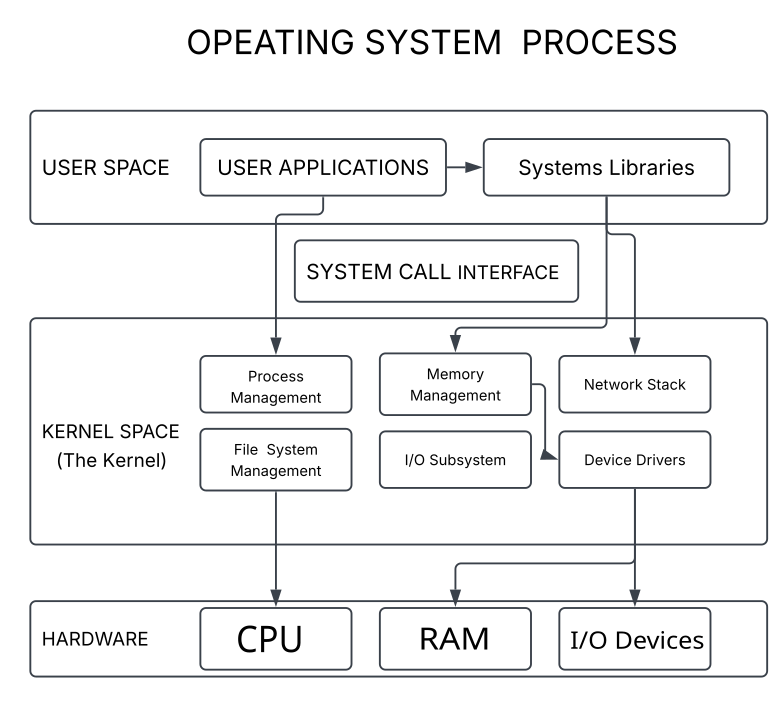
\includegraphics[width=0.7\textwidth]{os_process.png}
    \caption{Operating System Architecture Layers}
    \label{fig:os_process}
\end{figure}

\section{Discussion}
The representations above highlight the immense complexity hidden beneath a standard computing interface. To demystify the algorithmic logic presented in the working section, the OS boot sequence can be understood through this simple explanation:

When we switch on the computer, the CPU starts, and the system first performs POST, which checks whether the basic hardware is working properly.
\begin{itemize}
    \item \textbf{If hardware fails $\rightarrow$} the system stops and shows an error.
    \item \textbf{If everything is fine $\rightarrow$} the system finds the boot device, like an SSD/HDD.
\end{itemize}
It then loads and runs the bootloader. The bootloader loads the OS kernel into RAM and gives control to it. The kernel initializes drivers, memory, and the root filesystem. Then it starts necessary background services (daemons). Finally, the system starts the GUI or CLI, allowing the user to interact with the computer.

Beyond the boot sequence, the core responsibilities derived from the OS architecture include:
\begin{itemize}
    \item \textbf{Process Management:} Creating, suspending, scheduling, and terminating software processes.
    \item \textbf{Memory Management:} Tracking available RAM and securely allocating it to active applications.
    \item \textbf{File System Management:} Organizing directories, writing data to storage, and enforcing file permissions.
    \item \textbf{Device Management:} Using drivers to facilitate seamless communication between the software and physical peripherals.
\end{itemize}

\section{Conclusion}
The operating system is a highly orchestrated, event-driven resource manager that bridges the gap between physical hardware limitations and user application demands. Through a highly structured boot sequence and strict architectural layering, the OS successfully provides a continuous, stable, and secure computing environment.

% ==========================================
% STAGE 7: REFERENCES
% ==========================================
\begin{thebibliography}{9}

\bibitem{silberschatz} 
Abraham Silberschatz, Peter B. Galvin, and Greg Gagne, 
\textit{Operating System Concepts}, 10th ed. Hoboken, NJ: Wiley, 2018.

\bibitem{tanenbaum} 
Andrew S. Tanenbaum and Herbert Bos, 
\textit{Modern Operating Systems}, 4th ed. Pearson, 2014.

\bibitem{love} 
Robert Love, 
\textit{Linux Kernel Development}, 3rd ed. Addison-Wesley Professional, 2010.

\end{thebibliography}

\end{document}